\documentclass[twoside]{book}

% Packages required by doxygen
\usepackage{fixltx2e}
\usepackage{calc}
\usepackage{doxygen}
\usepackage[export]{adjustbox} % also loads graphicx
\usepackage{graphicx}
\usepackage[utf8]{inputenc}
\usepackage{makeidx}
\usepackage{multicol}
\usepackage{multirow}
\PassOptionsToPackage{warn}{textcomp}
\usepackage{textcomp}
\usepackage[nointegrals]{wasysym}
\usepackage[table]{xcolor}

% Font selection
\usepackage[T1]{fontenc}
\usepackage[scaled=.90]{helvet}
\usepackage{courier}
\usepackage{amssymb}
\usepackage{sectsty}
\renewcommand{\familydefault}{\sfdefault}
\allsectionsfont{%
  \fontseries{bc}\selectfont%
  \color{darkgray}%
}
\renewcommand{\DoxyLabelFont}{%
  \fontseries{bc}\selectfont%
  \color{darkgray}%
}
\newcommand{\+}{\discretionary{\mbox{\scriptsize$\hookleftarrow$}}{}{}}

% Page & text layout
\usepackage{geometry}
\geometry{%
  a4paper,%
  top=2.5cm,%
  bottom=2.5cm,%
  left=2.5cm,%
  right=2.5cm%
}
\tolerance=750
\hfuzz=15pt
\hbadness=750
\setlength{\emergencystretch}{15pt}
\setlength{\parindent}{0cm}
\setlength{\parskip}{3ex plus 2ex minus 2ex}
\makeatletter
\renewcommand{\paragraph}{%
  \@startsection{paragraph}{4}{0ex}{-1.0ex}{1.0ex}{%
    \normalfont\normalsize\bfseries\SS@parafont%
  }%
}
\renewcommand{\subparagraph}{%
  \@startsection{subparagraph}{5}{0ex}{-1.0ex}{1.0ex}{%
    \normalfont\normalsize\bfseries\SS@subparafont%
  }%
}
\makeatother

% Headers & footers
\usepackage{fancyhdr}
\pagestyle{fancyplain}
\fancyhead[LE]{\fancyplain{}{\bfseries\thepage}}
\fancyhead[CE]{\fancyplain{}{}}
\fancyhead[RE]{\fancyplain{}{\bfseries\leftmark}}
\fancyhead[LO]{\fancyplain{}{\bfseries\rightmark}}
\fancyhead[CO]{\fancyplain{}{}}
\fancyhead[RO]{\fancyplain{}{\bfseries\thepage}}
\fancyfoot[LE]{\fancyplain{}{}}
\fancyfoot[CE]{\fancyplain{}{}}
\fancyfoot[RE]{\fancyplain{}{\bfseries\scriptsize Generated by Doxygen }}
\fancyfoot[LO]{\fancyplain{}{\bfseries\scriptsize Generated by Doxygen }}
\fancyfoot[CO]{\fancyplain{}{}}
\fancyfoot[RO]{\fancyplain{}{}}
\renewcommand{\footrulewidth}{0.4pt}
\renewcommand{\chaptermark}[1]{%
  \markboth{#1}{}%
}
\renewcommand{\sectionmark}[1]{%
  \markright{\thesection\ #1}%
}

% Indices & bibliography
\usepackage{natbib}
\usepackage[titles]{tocloft}
\setcounter{tocdepth}{3}
\setcounter{secnumdepth}{5}
\makeindex

% Hyperlinks (required, but should be loaded last)
\usepackage{ifpdf}
\ifpdf
  \usepackage[pdftex,pagebackref=true]{hyperref}
\else
  \usepackage[ps2pdf,pagebackref=true]{hyperref}
\fi
\hypersetup{%
  colorlinks=true,%
  linkcolor=blue,%
  citecolor=blue,%
  unicode%
}

% Custom commands
\newcommand{\clearemptydoublepage}{%
  \newpage{\pagestyle{empty}\cleardoublepage}%
}

\usepackage{caption}
\captionsetup{labelsep=space,justification=centering,font={bf},singlelinecheck=off,skip=4pt,position=top}

%===== C O N T E N T S =====

\begin{document}

% Titlepage & ToC
\hypersetup{pageanchor=false,
             bookmarksnumbered=true,
             pdfencoding=unicode
            }
\pagenumbering{alph}
\begin{titlepage}
\vspace*{7cm}
\begin{center}%
{\Large Ultimate Tic Tac Toe }\\
\vspace*{1cm}
{\large Generated by Doxygen 1.8.12}\\
\end{center}
\end{titlepage}
\clearemptydoublepage
\pagenumbering{roman}
\tableofcontents
\clearemptydoublepage
\pagenumbering{arabic}
\hypersetup{pageanchor=true}

%--- Begin generated contents ---
\chapter{Intelligent Ultimate Tic-\/\+Tac-\/\+Toe playing bot}
\label{md___users_abhinavmoudgil_ut3-ai__r_e_a_d_m_e}
\hypertarget{md___users_abhinavmoudgil_ut3-ai__r_e_a_d_m_e}{}
Python implementation of Alpha Beta Pruning algorithm 
\chapter{Namespace Index}
\section{Namespace List}
Here is a list of all documented namespaces with brief descriptions\+:\begin{DoxyCompactList}
\item\contentsline{section}{\hyperlink{namespacesimulator}{simulator} }{\pageref{namespacesimulator}}{}
\item\contentsline{section}{\hyperlink{namespaceteam14}{team14} }{\pageref{namespaceteam14}}{}
\end{DoxyCompactList}

\chapter{Hierarchical Index}
\section{Class Hierarchy}
This inheritance list is sorted roughly, but not completely, alphabetically\+:\begin{DoxyCompactList}
\item Exception\begin{DoxyCompactList}
\item \contentsline{section}{simulator.\+Timed\+Out\+Exc}{\pageref{classsimulator_1_1_timed_out_exc}}{}
\end{DoxyCompactList}
\item \contentsline{section}{simulator.\+Manual\+\_\+player}{\pageref{classsimulator_1_1_manual__player}}{}
\item object\begin{DoxyCompactList}
\item \contentsline{section}{team14.\+Player14}{\pageref{classteam14_1_1_player14}}{}
\end{DoxyCompactList}
\item \contentsline{section}{simulator.\+Player1}{\pageref{classsimulator_1_1_player1}}{}
\item \contentsline{section}{simulator.\+Player2}{\pageref{classsimulator_1_1_player2}}{}
\end{DoxyCompactList}

\chapter{Class Index}
\section{Class List}
Here are the classes, structs, unions and interfaces with brief descriptions\+:\begin{DoxyCompactList}
\item\contentsline{section}{\hyperlink{classsimulator_1_1_manual__player}{simulator.\+Manual\+\_\+player} }{\pageref{classsimulator_1_1_manual__player}}{}
\item\contentsline{section}{\hyperlink{classsimulator_1_1_player1}{simulator.\+Player1} }{\pageref{classsimulator_1_1_player1}}{}
\item\contentsline{section}{\hyperlink{classteam14_1_1_player14}{team14.\+Player14} }{\pageref{classteam14_1_1_player14}}{}
\item\contentsline{section}{\hyperlink{classsimulator_1_1_player2}{simulator.\+Player2} }{\pageref{classsimulator_1_1_player2}}{}
\item\contentsline{section}{\hyperlink{classsimulator_1_1_timed_out_exc}{simulator.\+Timed\+Out\+Exc} }{\pageref{classsimulator_1_1_timed_out_exc}}{}
\end{DoxyCompactList}

\chapter{Namespace Documentation}
\hypertarget{namespacesimulator}{}\section{simulator Namespace Reference}
\label{namespacesimulator}\index{simulator@{simulator}}
\subsection*{Classes}
\begin{DoxyCompactItemize}
\item 
class \hyperlink{classsimulator_1_1_manual__player}{Manual\+\_\+player}
\item 
class \hyperlink{classsimulator_1_1_player1}{Player1}
\item 
class \hyperlink{classsimulator_1_1_player2}{Player2}
\item 
class \hyperlink{classsimulator_1_1_timed_out_exc}{Timed\+Out\+Exc}
\end{DoxyCompactItemize}
\subsection*{Functions}
\begin{DoxyCompactItemize}
\item 
def {\bfseries handler} (signum, frame)\hypertarget{namespacesimulator_a46f8d8f28740495ed8d5b41ea437dcb4}{}\label{namespacesimulator_a46f8d8f28740495ed8d5b41ea437dcb4}

\item 
def {\bfseries get\+\_\+init\+\_\+board\+\_\+and\+\_\+blockstatus} ()\hypertarget{namespacesimulator_a8e45993e8444b066b05673131b158973}{}\label{namespacesimulator_a8e45993e8444b066b05673131b158973}

\item 
def {\bfseries verification\+\_\+fails\+\_\+board} (board\+\_\+game, temp\+\_\+board\+\_\+state)\hypertarget{namespacesimulator_a3adefd4f4546beaf1d94585c78e85a82}{}\label{namespacesimulator_a3adefd4f4546beaf1d94585c78e85a82}

\item 
def {\bfseries verification\+\_\+fails\+\_\+block} (block\+\_\+stat, temp\+\_\+block\+\_\+stat)\hypertarget{namespacesimulator_a5253b1378b135994092a20df7de18273}{}\label{namespacesimulator_a5253b1378b135994092a20df7de18273}

\item 
def {\bfseries get\+\_\+empty\+\_\+out\+\_\+of} (gameb, blal, block\+\_\+stat)\hypertarget{namespacesimulator_ada9d7d7d9212b14a7afd6e15f4cabb34}{}\label{namespacesimulator_ada9d7d7d9212b14a7afd6e15f4cabb34}

\item 
def {\bfseries check\+\_\+valid\+\_\+move} (game\+\_\+board, block\+\_\+stat, current\+\_\+move, old\+\_\+move)\hypertarget{namespacesimulator_a67b5cc82640109b7cc386627b5613604}{}\label{namespacesimulator_a67b5cc82640109b7cc386627b5613604}

\item 
def {\bfseries update\+\_\+lists} (game\+\_\+board, block\+\_\+stat, move\+\_\+ret, fl)\hypertarget{namespacesimulator_a5b33c2bde7e0b8345b2390f6856e2891}{}\label{namespacesimulator_a5b33c2bde7e0b8345b2390f6856e2891}

\item 
def {\bfseries terminal\+\_\+state\+\_\+reached} (game\+\_\+board, block\+\_\+stat)\hypertarget{namespacesimulator_a6053b210441089cd163978de2542aa26}{}\label{namespacesimulator_a6053b210441089cd163978de2542aa26}

\item 
def {\bfseries decide\+\_\+winner\+\_\+and\+\_\+get\+\_\+message} (player, status, message)\hypertarget{namespacesimulator_a7cd222b72823285f1599e00edbc5321a}{}\label{namespacesimulator_a7cd222b72823285f1599e00edbc5321a}

\item 
def {\bfseries print\+\_\+lists} (gb, bs)\hypertarget{namespacesimulator_a41eeaf13839dd5ee2637c87b29e91d1a}{}\label{namespacesimulator_a41eeaf13839dd5ee2637c87b29e91d1a}

\item 
def {\bfseries simulate} (\hyperlink{namespacesimulator_a0959268797d7e20ce30ad540652df09c}{obj1}, obj2)\hypertarget{namespacesimulator_a655a7bd5141e96e66d3955394af60234}{}\label{namespacesimulator_a655a7bd5141e96e66d3955394af60234}

\end{DoxyCompactItemize}
\subsection*{Variables}
\begin{DoxyCompactItemize}
\item 
int {\bfseries inf} = 1\hypertarget{namespacesimulator_a3fec35fa935a5c32d8588b1493526364}{}\label{namespacesimulator_a3fec35fa935a5c32d8588b1493526364}

\item 
string \hyperlink{namespacesimulator_a0959268797d7e20ce30ad540652df09c}{obj1} = \textquotesingle{}\textquotesingle{}\hypertarget{namespacesimulator_a0959268797d7e20ce30ad540652df09c}{}\label{namespacesimulator_a0959268797d7e20ce30ad540652df09c}

\begin{DoxyCompactList}\small\item\em get game playing objects \end{DoxyCompactList}\item 
string {\bfseries obj2} = \textquotesingle{}\textquotesingle{}\hypertarget{namespacesimulator_aa3d45be0f080d6af27999657e50e7674}{}\label{namespacesimulator_aa3d45be0f080d6af27999657e50e7674}

\item 
{\bfseries option} = sys.\+argv\mbox{[}1\mbox{]}\hypertarget{namespacesimulator_aecffc3da633925ffc656e91c5888008b}{}\label{namespacesimulator_aecffc3da633925ffc656e91c5888008b}

\item 
{\bfseries num} = random.\+uniform(0,1)\hypertarget{namespacesimulator_a05c130ea7b953857514cba6eb9ee710f}{}\label{namespacesimulator_a05c130ea7b953857514cba6eb9ee710f}

\end{DoxyCompactItemize}


\subsection{Detailed Description}
\begin{DoxyVerb}A Python simuation of Ultimate Tic Tac Toe
Player 2 - AI test player 1 
Player 1 - AI test player 2
Manual   - Manual user player
\end{DoxyVerb}
 
\hypertarget{namespaceteam14}{}\section{team14 Namespace Reference}
\label{namespaceteam14}\index{team14@{team14}}
\subsection*{Classes}
\begin{DoxyCompactItemize}
\item 
class \hyperlink{classteam14_1_1_player14}{Player14}
\end{DoxyCompactItemize}
\subsection*{Variables}
\begin{DoxyCompactItemize}
\item 
int {\bfseries inf} = 1\hypertarget{namespaceteam14_ab1927b8ab2a2ee77dc0d8626baeb6afd}{}\label{namespaceteam14_ab1927b8ab2a2ee77dc0d8626baeb6afd}

\end{DoxyCompactItemize}


\subsection{Detailed Description}
\begin{DoxyVerb}Python implementation of Alpha Beta Pruning AI algorithm
\end{DoxyVerb}
 
\chapter{Class Documentation}
\hypertarget{classsimulator_1_1_manual__player}{}\section{simulator.\+Manual\+\_\+player Class Reference}
\label{classsimulator_1_1_manual__player}\index{simulator.\+Manual\+\_\+player@{simulator.\+Manual\+\_\+player}}
\subsection*{Public Member Functions}
\begin{DoxyCompactItemize}
\item 
def {\bfseries \+\_\+\+\_\+init\+\_\+\+\_\+} (self)\hypertarget{classsimulator_1_1_manual__player_a7ad3ae722a30179456c3aaa99723e691}{}\label{classsimulator_1_1_manual__player_a7ad3ae722a30179456c3aaa99723e691}

\item 
def {\bfseries move} (self, temp\+\_\+board, temp\+\_\+block, old\+\_\+move, flag)\hypertarget{classsimulator_1_1_manual__player_a1668ba6e718ba103b78734ac520d8de2}{}\label{classsimulator_1_1_manual__player_a1668ba6e718ba103b78734ac520d8de2}

\end{DoxyCompactItemize}


The documentation for this class was generated from the following file\+:\begin{DoxyCompactItemize}
\item 
/\+Users/abhinavmoudgil/ut3-\/ai/simulator.\+py\end{DoxyCompactItemize}

\hypertarget{classsimulator_1_1_player1}{}\section{simulator.\+Player1 Class Reference}
\label{classsimulator_1_1_player1}\index{simulator.\+Player1@{simulator.\+Player1}}
\subsection*{Public Member Functions}
\begin{DoxyCompactItemize}
\item 
def {\bfseries \+\_\+\+\_\+init\+\_\+\+\_\+} (self)\hypertarget{classsimulator_1_1_player1_aed6db868228e85cd0b764eb8f48fef85}{}\label{classsimulator_1_1_player1_aed6db868228e85cd0b764eb8f48fef85}

\item 
def {\bfseries move} (self, temp\+\_\+board, temp\+\_\+block, old\+\_\+move, flag)\hypertarget{classsimulator_1_1_player1_a1077336392acb292bf66e255c92de40d}{}\label{classsimulator_1_1_player1_a1077336392acb292bf66e255c92de40d}

\end{DoxyCompactItemize}
\subsection*{Static Public Attributes}
\begin{DoxyCompactItemize}
\item 
{\bfseries cells} = get\+\_\+empty\+\_\+out\+\_\+of(temp\+\_\+board, blocks\+\_\+allowed,temp\+\_\+block)\hypertarget{classsimulator_1_1_player1_a8a2c5625304540c68ac00037392f6a56}{}\label{classsimulator_1_1_player1_a8a2c5625304540c68ac00037392f6a56}

\end{DoxyCompactItemize}


The documentation for this class was generated from the following file\+:\begin{DoxyCompactItemize}
\item 
/\+Users/abhinavmoudgil/ut3-\/ai/simulator.\+py\end{DoxyCompactItemize}

\hypertarget{classteam14_1_1_player14}{}\section{team14.\+Player14 Class Reference}
\label{classteam14_1_1_player14}\index{team14.\+Player14@{team14.\+Player14}}
Inheritance diagram for team14.\+Player14\+:\begin{figure}[H]
\begin{center}
\leavevmode
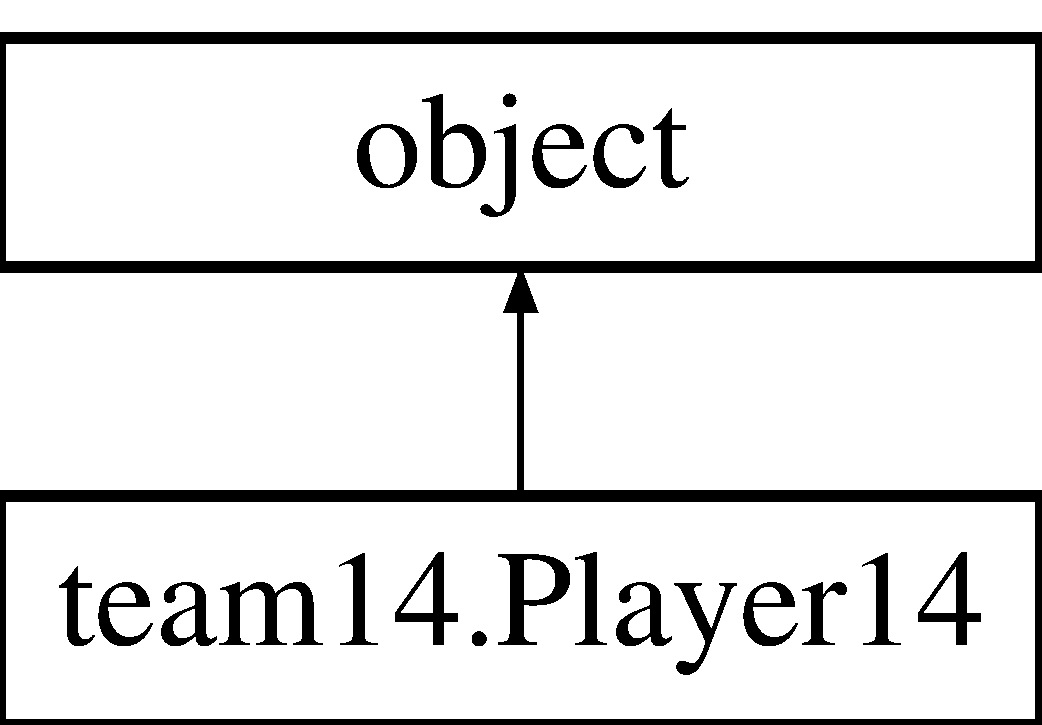
\includegraphics[height=2.000000cm]{classteam14_1_1_player14}
\end{center}
\end{figure}
\subsection*{Public Member Functions}
\begin{DoxyCompactItemize}
\item 
def {\bfseries \+\_\+\+\_\+init\+\_\+\+\_\+} (self)\hypertarget{classteam14_1_1_player14_aa4c4501ba539b6047c5605f8d8b691ba}{}\label{classteam14_1_1_player14_aa4c4501ba539b6047c5605f8d8b691ba}

\item 
def {\bfseries move} (self, current\+\_\+board\+\_\+game, board\+\_\+stat, move\+\_\+by\+\_\+opponent, flag)\hypertarget{classteam14_1_1_player14_a3c576d13c4fd3cbebe07410937c522a1}{}\label{classteam14_1_1_player14_a3c576d13c4fd3cbebe07410937c522a1}

\item 
def {\bfseries get\+Opp} (self, flag)\hypertarget{classteam14_1_1_player14_ad0111ea694d975f6d62d71266f5b5c25}{}\label{classteam14_1_1_player14_ad0111ea694d975f6d62d71266f5b5c25}

\item 
def {\bfseries get\+Valid\+Cells} (self, current\+\_\+board\+\_\+game, board\+\_\+stat, move\+\_\+by\+\_\+opponent)\hypertarget{classteam14_1_1_player14_a113eb0d90ab81e3faf8dca1ab6e0fe14}{}\label{classteam14_1_1_player14_a113eb0d90ab81e3faf8dca1ab6e0fe14}

\item 
def {\bfseries update\+Board\+Stat} (self, board\+\_\+game, board\+\_\+stat, move, flag)\hypertarget{classteam14_1_1_player14_afb40cef5383017eb5c6c38e3bf729b31}{}\label{classteam14_1_1_player14_afb40cef5383017eb5c6c38e3bf729b31}

\item 
def {\bfseries alpha\+Beta\+Pruning} (self, board\+\_\+game, board\+\_\+stat, depth, alpha, beta, flag, node)\hypertarget{classteam14_1_1_player14_a05464411351104bdef64e927194d0174}{}\label{classteam14_1_1_player14_a05464411351104bdef64e927194d0174}

\item 
def {\bfseries is\+Terminal} (self, board\+\_\+stat)\hypertarget{classteam14_1_1_player14_aac4b143e5c11707b66e093cd0c09f81c}{}\label{classteam14_1_1_player14_aac4b143e5c11707b66e093cd0c09f81c}

\item 
def {\bfseries get\+Utility\+Val} (self, board\+\_\+stat)\hypertarget{classteam14_1_1_player14_a048f6817a22e7e7a1e56716cf91becad}{}\label{classteam14_1_1_player14_a048f6817a22e7e7a1e56716cf91becad}

\item 
def {\bfseries get\+Heuristic\+Val} (self, board\+\_\+game, board\+\_\+stat)\hypertarget{classteam14_1_1_player14_a161f310aacad9d80e7ddf305708663b0}{}\label{classteam14_1_1_player14_a161f310aacad9d80e7ddf305708663b0}

\item 
def {\bfseries generate\+Heuristic\+Matrix} (self)\hypertarget{classteam14_1_1_player14_ac64fa497477b4fe863a3651cd4f8bb8e}{}\label{classteam14_1_1_player14_ac64fa497477b4fe863a3651cd4f8bb8e}

\end{DoxyCompactItemize}
\subsection*{Public Attributes}
\begin{DoxyCompactItemize}
\item 
{\bfseries inf}\hypertarget{classteam14_1_1_player14_a136abdac239c3735bfa83c339d792229}{}\label{classteam14_1_1_player14_a136abdac239c3735bfa83c339d792229}

\item 
{\bfseries my\+Mark}\hypertarget{classteam14_1_1_player14_a1d4908c0520c91ed8b5edb9c2daa7d5d}{}\label{classteam14_1_1_player14_a1d4908c0520c91ed8b5edb9c2daa7d5d}

\item 
{\bfseries other}\hypertarget{classteam14_1_1_player14_a90067b2bdb658928edcff42c7966b646}{}\label{classteam14_1_1_player14_a90067b2bdb658928edcff42c7966b646}

\item 
{\bfseries node\+\_\+count}\hypertarget{classteam14_1_1_player14_ae2891829e4cdeac5c6c5c9cf660aaa3b}{}\label{classteam14_1_1_player14_ae2891829e4cdeac5c6c5c9cf660aaa3b}

\item 
{\bfseries representative\+\_\+three\+\_\+matrix}\hypertarget{classteam14_1_1_player14_a531e2db0254a00ddee7daa3c9483aed5}{}\label{classteam14_1_1_player14_a531e2db0254a00ddee7daa3c9483aed5}

\item 
{\bfseries heuristic\+\_\+value\+\_\+matrix}\hypertarget{classteam14_1_1_player14_aa6c8b1b97337e945538b700bb3d544c9}{}\label{classteam14_1_1_player14_aa6c8b1b97337e945538b700bb3d544c9}

\end{DoxyCompactItemize}


The documentation for this class was generated from the following file\+:\begin{DoxyCompactItemize}
\item 
/\+Users/abhinavmoudgil/ut3-\/ai/team14.\+py\end{DoxyCompactItemize}

\hypertarget{classsimulator_1_1_player2}{}\section{simulator.\+Player2 Class Reference}
\label{classsimulator_1_1_player2}\index{simulator.\+Player2@{simulator.\+Player2}}
\subsection*{Public Member Functions}
\begin{DoxyCompactItemize}
\item 
def {\bfseries \+\_\+\+\_\+init\+\_\+\+\_\+} (self)\hypertarget{classsimulator_1_1_player2_a11323b9675fca456c353ef27423d8e6e}{}\label{classsimulator_1_1_player2_a11323b9675fca456c353ef27423d8e6e}

\item 
def {\bfseries move} (self, temp\+\_\+board, temp\+\_\+block, old\+\_\+move, flag)\hypertarget{classsimulator_1_1_player2_a2b8c0b33bac443b650d67b7ed9d3cf40}{}\label{classsimulator_1_1_player2_a2b8c0b33bac443b650d67b7ed9d3cf40}

\end{DoxyCompactItemize}
\subsection*{Static Public Attributes}
\begin{DoxyCompactItemize}
\item 
{\bfseries cells} = get\+\_\+empty\+\_\+out\+\_\+of(temp\+\_\+board,blocks\+\_\+allowed,temp\+\_\+block)\hypertarget{classsimulator_1_1_player2_a4dd86490ce0d9295470db52ce7160159}{}\label{classsimulator_1_1_player2_a4dd86490ce0d9295470db52ce7160159}

\end{DoxyCompactItemize}


The documentation for this class was generated from the following file\+:\begin{DoxyCompactItemize}
\item 
/\+Users/abhinavmoudgil/ut3-\/ai/simulator.\+py\end{DoxyCompactItemize}

\hypertarget{classsimulator_1_1_timed_out_exc}{}\section{simulator.\+Timed\+Out\+Exc Class Reference}
\label{classsimulator_1_1_timed_out_exc}\index{simulator.\+Timed\+Out\+Exc@{simulator.\+Timed\+Out\+Exc}}
Inheritance diagram for simulator.\+Timed\+Out\+Exc\+:\begin{figure}[H]
\begin{center}
\leavevmode
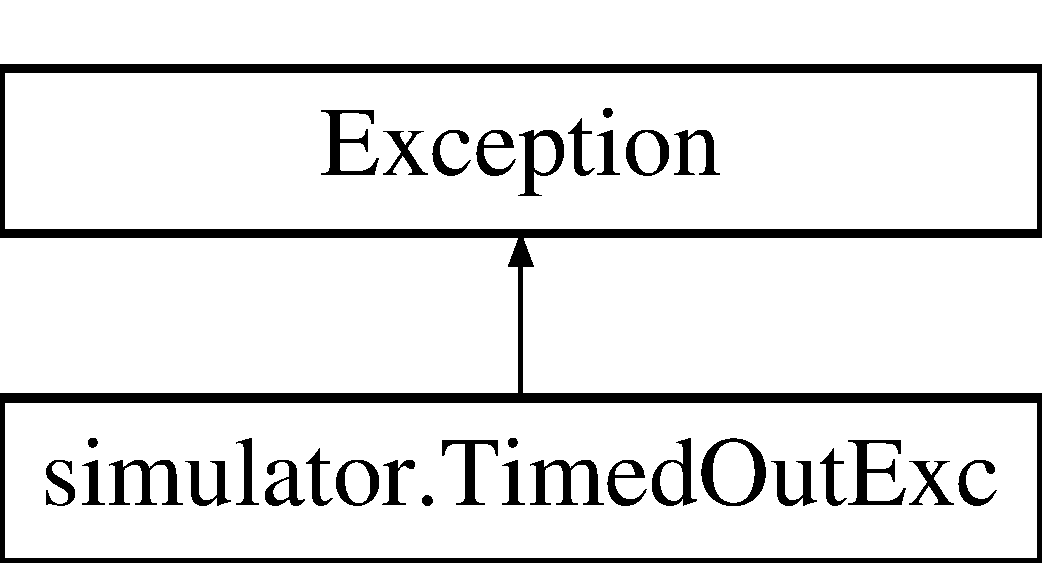
\includegraphics[height=2.000000cm]{classsimulator_1_1_timed_out_exc}
\end{center}
\end{figure}


The documentation for this class was generated from the following file\+:\begin{DoxyCompactItemize}
\item 
/\+Users/abhinavmoudgil/ut3-\/ai/simulator.\+py\end{DoxyCompactItemize}

%--- End generated contents ---

% Index
\backmatter
\newpage
\phantomsection
\clearemptydoublepage
\addcontentsline{toc}{chapter}{Index}
\printindex

\end{document}
